% 宇宙的演化
%% 还需要插入预备知识等等

宇宙演化可以大约分为两个时期,(详见\autoref{UniEvo_tab1} \footnote{翻译自Daniel Baumann,TASI Lectures on Inflation, \href{https://arxiv.org/abs/0907.5424}{arXiv:0907.5424},1.2 节,Table1}),从创世之初($t=0$) 到创世后3分钟我们可以称为前物质时期.这个时期可以大致分为两个时期:从宇宙诞生后到$10^{-43}$秒,此时宇宙沐浴于 $10^{18}\Si{GeV}$ 的高温中,四大相互作用被统一在一起.随后到$10^{-34}$秒宇宙在高温中经历\textbf{暴涨(Inflation)},宇宙尺度因子迅速扩大(详见\autoref{UniEvo_fig1} \footnote{引自 Daniel Baumann,TASI Lectures on Inflation, \href{https://arxiv.org/abs/0907.5424}{arXiv:0907.5424},1.2 节,Figure2}).在暴涨快结束时超对称破缺,宇宙中的重元素开始产生.

\begin{table}[ht]
\centering
\caption{宇宙大事记(问号表示理论尚未给出合理解释)}\label{UniEvo_tab1}
\begin{tabular}{|r|r|r|}
\hline
 & 时间 & 能量 \\
\hline
普朗克时间奇点? & $<10^{-43}\Si{s}$ & $10^{18}\Si{GeV}$ \\
\hline
弦论尺度?       & $>10^{-43}\Si{s}$ & $<10^{18}\Si{GeV}$ \\
\hline
超统一?         & $\sim 10^{-36}\Si{s}$ & $10^{15}\Si{GeV}$ \\
\hline
暴涨开始?       & $>10^{-34}\Si{s}$ & $<10^{15} \Si{GeV}$ \\
\hline
超对称破缺?     & $<10^{-10}\Si{s}$ & $>1 \Si{TeV}$ \\
\hline
重元素产生?     & $<10^{-10}\Si{s}$ & $>1 \Si{TeV}$ \\
\hline
电弱统一时期    & $10^{-10}\Si{s}$ & $1 \Si{TeV}$ \\
\hline
夸克-强子转换时期 & $10^{-4}\Si{s}$ & $10^2 \Si{MeV}$ \\
\hline
核子冷却        & $0.01\Si{s}$ & $10 \Si{MeV}$ \\
\hline
中微子退偶      & $1 \Si{s}$  & $1 \Si{MeV}$ \\
\hline
大爆炸原核初合成  & $3 \Si{min}$ & $0.1 \Si{MeV}$ \\
\hline
物质-辐射密度相等 & $10^4\Si{yrs}$  & $1 \Si{eV}$ \\
\hline
再融合 & $10^5\Si{yrs}$  & $0.1 \Si{eV}$ \\
\hline
宇宙黑暗时期 & $10^5 - 10^8\Si{yrs}$  &  \\
\hline
再电离 & $10^8\Si{yrs}$  &  \\
\hline
星系形成 & $\sim 6 \times 10^8\Si{yrs}$  &  \\
\hline
暗能量 & $\sim 10^9\Si{yrs}$  &  \\
\hline
太阳系形成 & $ \sim 8 \times 10^9\Si{yrs}$  &  \\
\hline
\end{tabular}
\end{table}

\begin{figure}[ht]
\centering
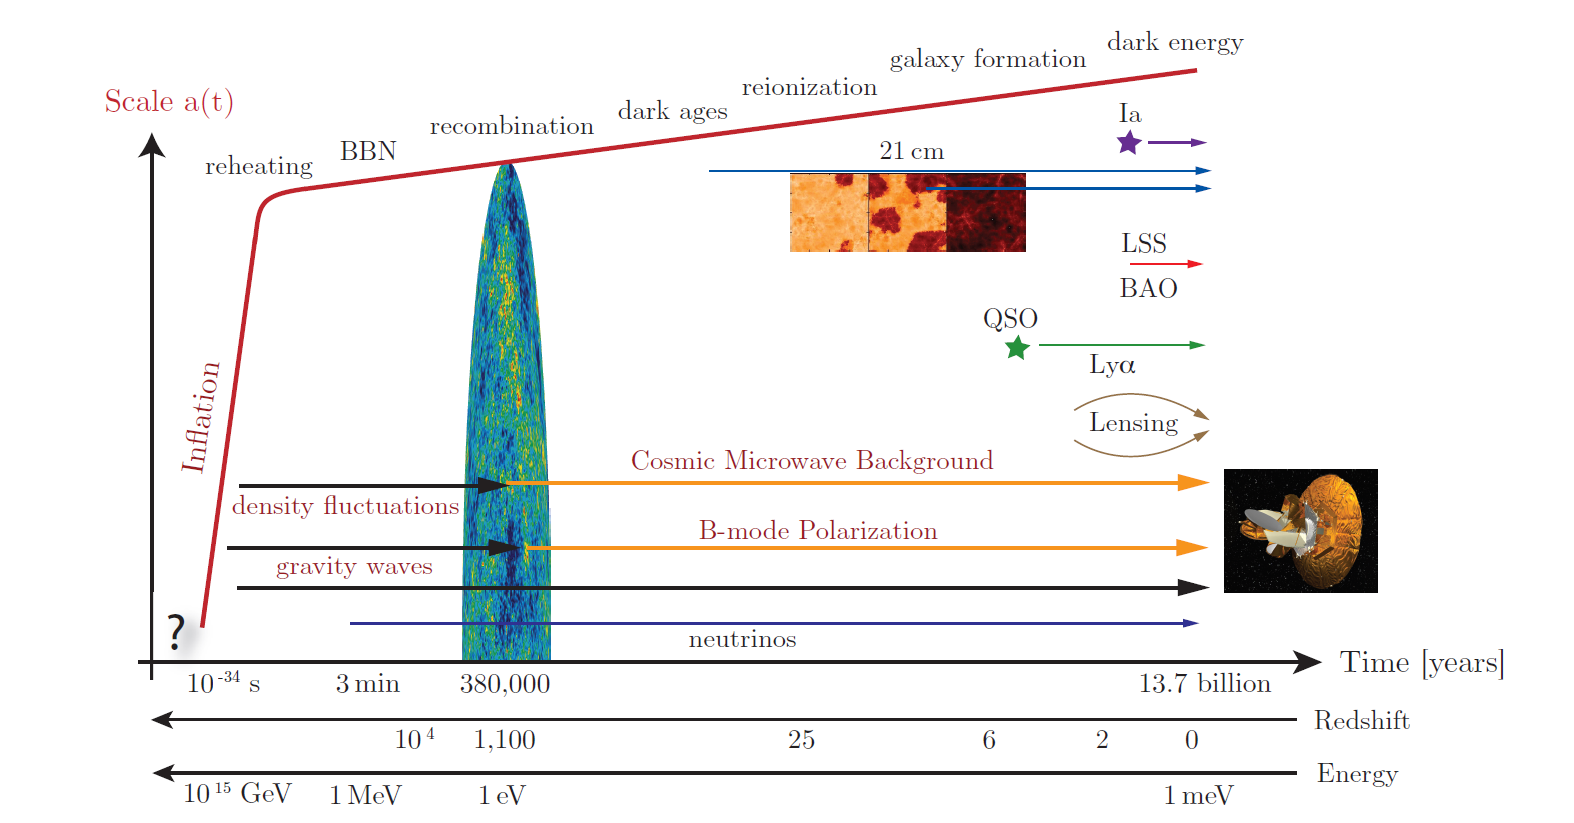
\includegraphics[width=14.25cm]{./figures/UniEvo_2.png}
\caption{宇宙尺度及成分表} \label{UniEvo_fig1}
\end{figure}

从$10^{-10}$ 秒到宇宙诞生后 3 分钟,宇宙暴涨结束,宇宙从$1\Si{TeV}$ 迅速逐渐冷却到 $0.1 \Si{MeV}$. 在此期间暴涨所释放的能量把宇宙重新加热,宇宙中的电弱相互作用开始分离,夸克结合成强子,中子冷却下来,宇宙中的核子开始在相互作用下结合并形成,称为\textbf{原核初合成}(BBN);中微子在创世后1秒与其他核子退耦并此后不再与其他物质产生相互作用,一直传播到现在.此时,宇宙开始以辐射为主导,我们也称为辐射主导时期的开始,此外,宇宙中的原初扰动和引力波开始形成.

\begin{figure}[ht]
\centering
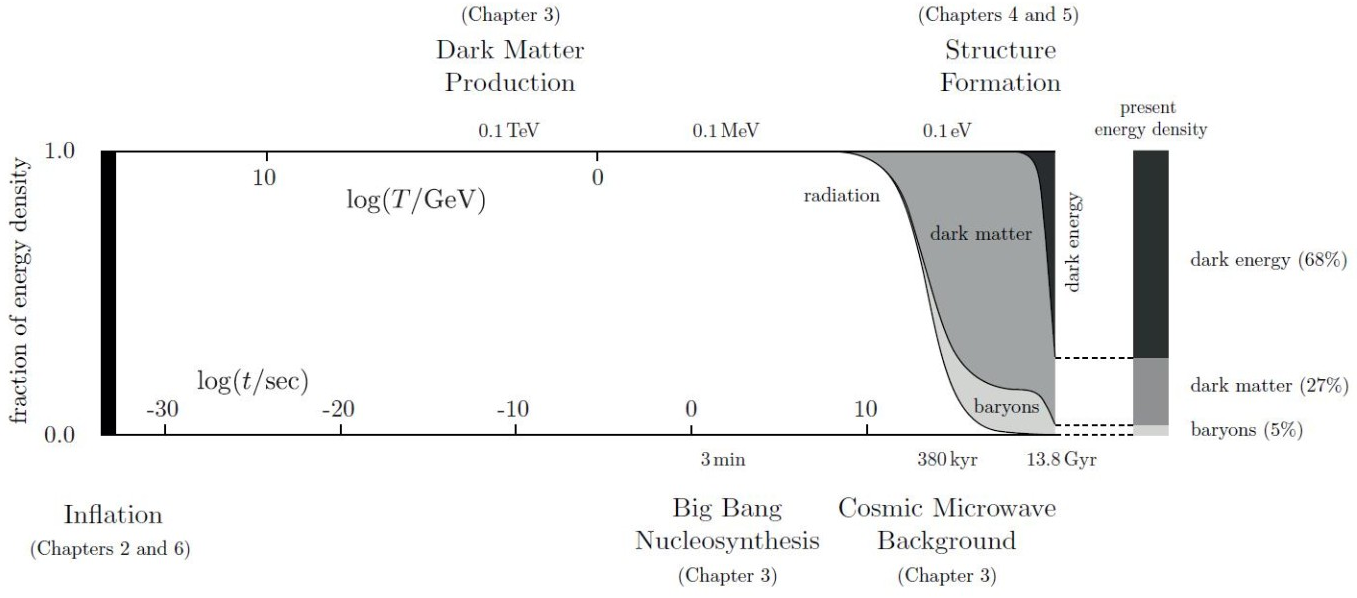
\includegraphics[width=14.25cm]{./figures/UniEvo_1.png}
\caption{宇宙成分变化} \label{UniEvo_fig2}
\end{figure}

从创世后3分钟到现在,我们可以称为后物质时期.我们也可以把这个时期大致地分为两个时期:从宇宙诞生后3分钟到380.000年,宇宙一直以辐射为主导(详见\autoref{UniEvo_fig2} \footnote{引自 Daniel Baumann,Cosmology,Perface,Figure 1}).随着宇宙的膨胀光子和物质从密度对等逐渐分离,且光子、物质和原初引力波进行充分的相互作用称为\textbf{再融合}(recombination),光子逐渐冷却下来形成\textbf{宇宙辐射背景}(CMB),期间暗物质开始形成.

从宇宙诞生后 $380.000$ 年到现在,宇宙进入物质主导时期,另一部分光子形成了宇宙辐射背景并随着时间演化到现在,一部分光子和原初引力波相互作用后成为B-模极化光子; 一部分原初引力波和中微子并不参与到相互作用中,并随着时间演化直到现在.在此期间,各大星系形成于创世后 $10^8$ 年之后,太阳系形成于 $8\times 10^9$ 年.
